%\documentclass[draft]{beamer}
\documentclass{beamer}

\usetheme{Warsaw}
\usecolortheme{seahorse}

\usepackage[utf8]{inputenc}
\usepackage[polish]{babel}
\usepackage{polski}
\usepackage{hyperref}
\usepackage{fancyhdr}
\usepackage{verbatim}

\newcommand{\strong}[1]{\begin{center}\LARGE{\textbf{#1}}\end{center}}

\newcommand{\terminalin}[2]{\small{\textbf{#1}\\\hspace{0.5cm}\tiny{\textsf{\textcolor{gray}{#2}}}} \\}
\newcommand{\terminalone}[1]{\small{\textbf{#1} \\}}

\hypersetup{linkbordercolor=1 1 1}

\title{Anomaly Intrusion Detection System}
\author[Michał Bugno \and Antoni Piechnik]
{
  \textbf{Michał Bugno} msq@student.agh.edu.pl \\
  \textbf{Antoni Piechnik} piechnik@student.agh.edu.pl
}
\date{\today}
\begin{document}
\maketitle

\section{Wstęp}

\subsection{IDS?}
\begin{frame}
  \frametitle{Intrusion Detection System}
  \begin{itemize}
    \item wykrywa niebezpieczne zachowania
    \begin{itemize}
      \item włamanie do systemu
      \item Denial of Service (atak na pewien ``zasób``)
      \item predefiniowane wzorce zachowań
    \end{itemize}
    \item podejmuje stosowane działania
    \begin{itemize}
      \item wyłączenie sieci
      \item wylogowanie użytkownika
      \item poinformowanie o zagrożeniu (mail?)
    \end{itemize}
  \end{itemize}
\end{frame}

\subsection{Rodzaje}
\begin{frame}
  \frametitle{Rodzaje}
  Typy systemów detekcji niebezpiecznych zachowań
  \begin{itemize}
    \item \textbf{anomaly} -- podejście ``algorytmiczne``
    \item \textbf{misuse} -- pojdeście ``pattern matching``
    \item \textbf{monitoring} -- pojdeście ``monitorowania celu``
    \item \ldots i ich kombinacje
  \end{itemize}
  Pierwsze podejście korzysta z algorytmów, aby wykryć czy mamy do
  czynienia z atakiem (problem fałszywych pozytywów a co gorsza fałszywych
  negatywów), drugie posiada pewien zestaw reguł, które definiują nam
  zagrożenia (problem nie zdefiniowania zagrożenia). Monitorowanie celu bada
  określone cele i w przypadku ataku informuje o nim (i/lub odwraca zmiany).
\end{frame}

\section{Anomaly IDS}

\subsection{Podejście statystyczne}
\begin{frame}
  \frametitle{Podejście statystyczne}
    \begin{figure}
      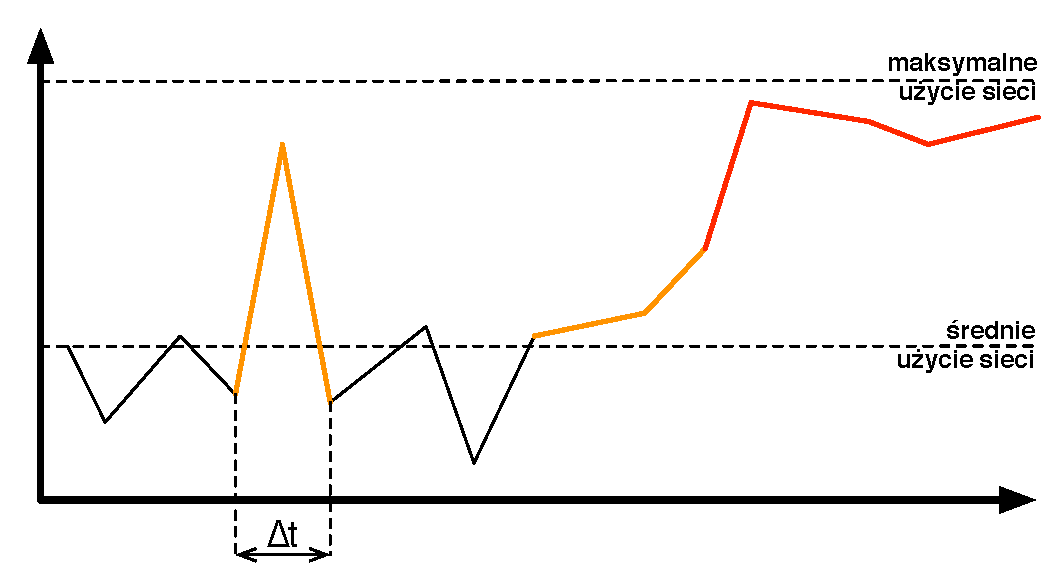
\includegraphics[width=20em]{network_usage.pdf}
      \caption{Podejście statystyczne do badania ataku sieciowego}
    \end{figure}
\end{frame}
\begin{frame}
  \frametitle{Podejście statystyczne}
  \begin{itemize}
    \item solidne podstawy statystyczne ułatwiają analizę
    \item nieczułe na kolejność zdarzeń
    \item możliwe fałszywe pozytywy/negatywy
  \end{itemize}
\end{frame}

\subsection{Przewidywanie wzorców}
\begin{frame}
  \frametitle{Przewidywanie wzorców}
    \begin{figure}
      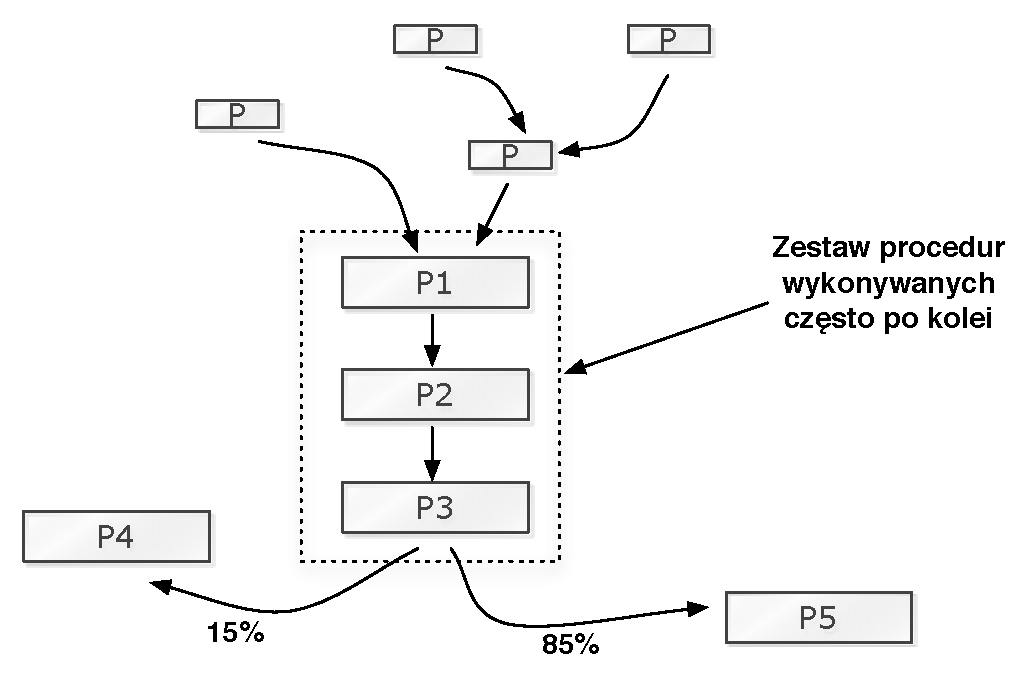
\includegraphics[width=20em]{procedure_execution.pdf}
      \caption{Przewidywanie wzorców w wywołaniu procedur}
    \end{figure}
\end{frame}
\begin{frame}
  \frametitle{Przewidywanie wzorców}
  \begin{itemize}
    \item niedostateczna ilość ``dobrych wzorców``
    \item użytkownicy często działają ``sekwencjami``
    \item wyznacza konkretne miejsca ataku
  \end{itemize}
\end{frame}

\subsection{Sieci neuronowe}
\begin{frame}
  \frametitle{Sieci neuronowe}
    \begin{figure}
      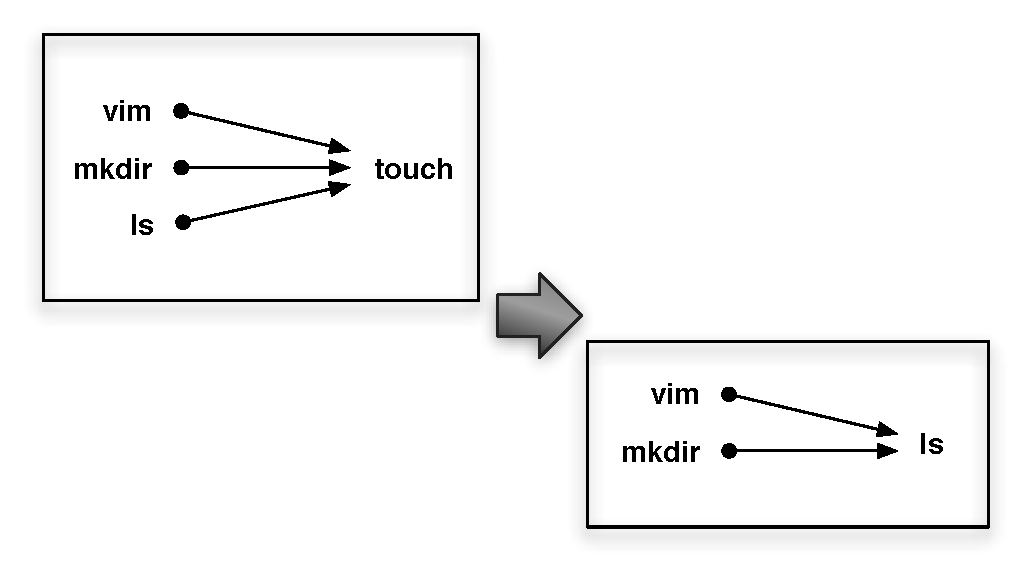
\includegraphics[width=20em]{neural_net.pdf}
      \caption{Tworzenie profilu użytkownika za pomocą sieci neuronowych}
    \end{figure}
\end{frame}
\begin{frame}
  \frametitle{Sieci neuronowe}
  \begin{itemize}
    \item znajdują ``różnice`` między profilem oczekiwanym a aktualnym (np.
        wywołania innych poleceń po sekwencji wywołań znanych)
    \item nie potrzebują założeń jak np. w podejściu statystycznym
    \item trudność w ustaleniu ostatnich \textbf{n} analizowanych poleceń
        (zbyt dużo niepotrzebnych danych vs zbyt mało znaczących informacji)
  \end{itemize}
\end{frame}

\subsection{Algorytmy genetyczne}
\begin{frame}
  \frametitle{Algorytmy genetyczne}
    \begin{figure}
      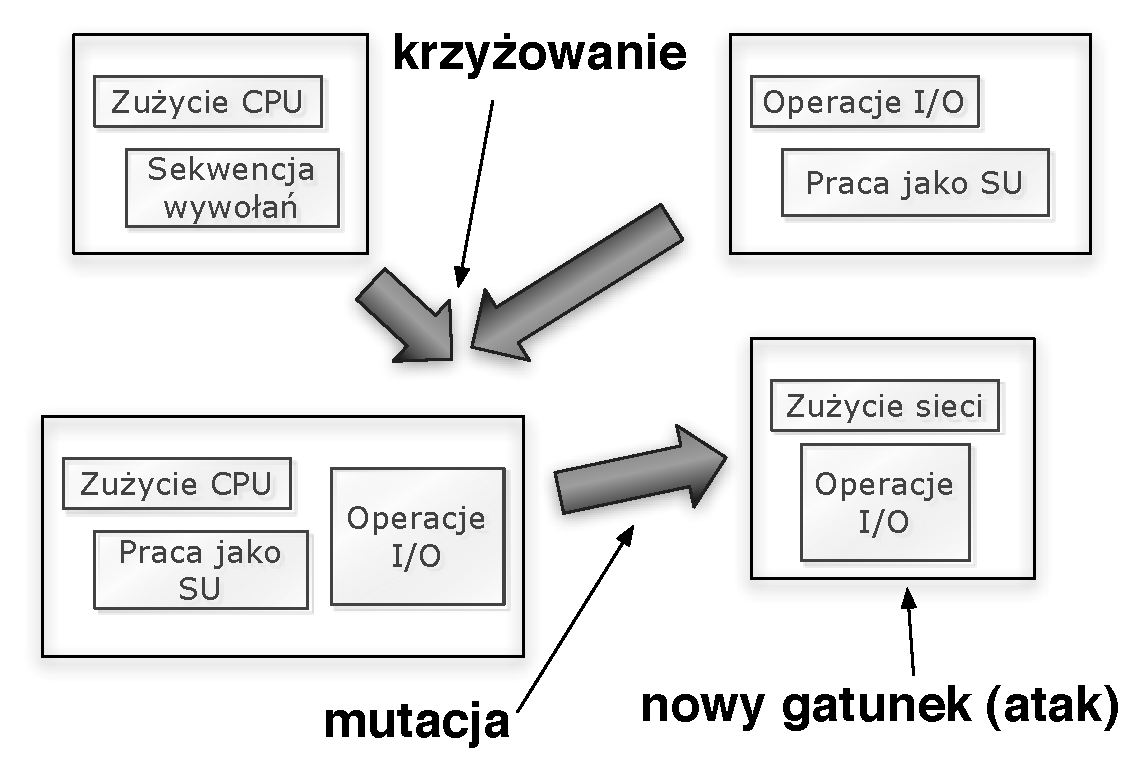
\includegraphics[width=20em]{genetic_algorithm.pdf}
      \caption{Przykład działania algorytmu genetycznego generującego nowy gatunek}
    \end{figure}
\end{frame}
\begin{frame}
  \frametitle{Algorytmy genetyczne}
  \begin{itemize}
    \item potrzebne ``wejście`` (gatunki potencjalnie niebezpieczne)
    \item dostosowuje się do nowych środowisk (nowych rodzajów ataków)
    \item mało prawdopodobne gatunki są usuwane, mutują ``niebezpieczne``
  \end{itemize}
\end{frame}

\section{Projekt}
\subsection{Cele}
\begin{frame}
  \frametitle{Cele projektu}
  \begin{itemize}
    \item znajdowanie sytuacji niebezpiecznych
    \item informowanie o wystąpieniu takich sytuacji
    \item automatyczne zapobieganie w przypadku gdy to możliwe
  \end{itemize}
\end{frame}

\subsection{Zasięg}
\begin{frame}
  \frametitle{Zasięg projektu}
  \begin{itemize}
    \item analiza przepływu danych sieciowych
    \item stworzenie profilu użytkownika przy pomocy omówionych narzędzi
    \item automatyzacja systemu (odcięcie sieci, wylogowanie użytkownika)
    \item informowanie o potencjalnym niebezpieczeństwie
    \item demon (niskie zużycie procesora)
    \item definiowane godziny działania
  \end{itemize}
\end{frame}

\section{Bibliografia}

\begin{frame}
  \frametitle{Bibliografia}
  \begin{itemize}
    \item \textit{Classification and Detection of Computer Intrusions}, Sandeep Kumar
    \item \textit{Systemy wykrywania intruzów}, Piotr Dorosz
    \item Internet :)
  \end{itemize}
\end{frame}



\end{document}
